\xpartbox{Abstract}

\begin{xpsectionbox}{}{}

\emph{\color{blue} NLM’s People Locator system allows the posting of photos and simple metadata (name, age, location) for persons missing (or found) in the wake of a disaster. To extend the current text-based search method to a visual search for people's faces, we developed FaceMatch, a system to match faces in a query image to those in the stored photos.
	Face matching is a two-stage process: faces in photos sent as queries are first localized using an improved Viola-Jones face detector, and then image features (SIFT, SURF, ORB and HAAR) are extracted, combined and matched against an index of features extracted from the stored photos. 
Face matching is challenging because of the lack of training data, low-resolution photos, wide variability in lighting, facial expression, head pose, ethnicity, occlusions and deformed faces due to injury.
	Ongoing research, using images collected from the 2010 earthquake in Haiti and Labeled Faces in the Wild dataset, includes exploring more discriminating features, modeling skin color for more accurate face localization, a Haar wavelet-based technique to eliminate near-duplicate photos, and image normalization. FaceMatch speed and accuracy performance results are presented.}

\end{xpsectionbox}

\begin{xpsectionbox}{Challenges}{}

\begin{minipage}{0.45\linewidth}
\begin{itemize}
	\item size of HEPL database is about $15$K images
	\item pictures may contain $0$, $1$, $2$, $\ldots N$ faces
	\item face-like objects (cats and dogs faces)
	\item query/database images may be of suboptimal quality due to
	\item partially occluded or damaged faces
	\item presence of duplicates and near-duplicates
	\item inconsistency due to facial hair, glasses, jewelry, aging
\end{itemize}
\end{minipage}
\begin{minipage}{0.55\linewidth}
\begin{center}

			\vspace{-1cm}
			
			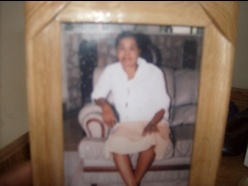
\includegraphics[height=0.22\linewidth]{images/PL_low_quality}
			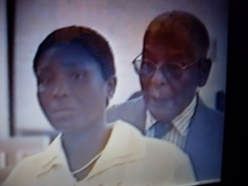
\includegraphics[height=0.22\linewidth]{images/HEPL_low_quality}
			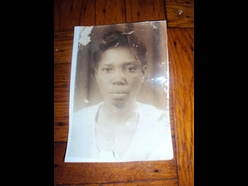
\includegraphics[height=0.22\linewidth]{images/HEPL_picture_photo}

			\vspace{0.2cm}			
			
			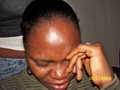
\includegraphics[height=0.22\linewidth]{images/HEPL_occlusion}
			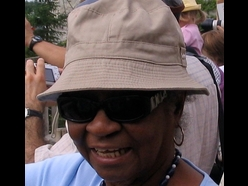
\includegraphics[height=0.22\linewidth]{images/HEPL_sunglasses_hat}
			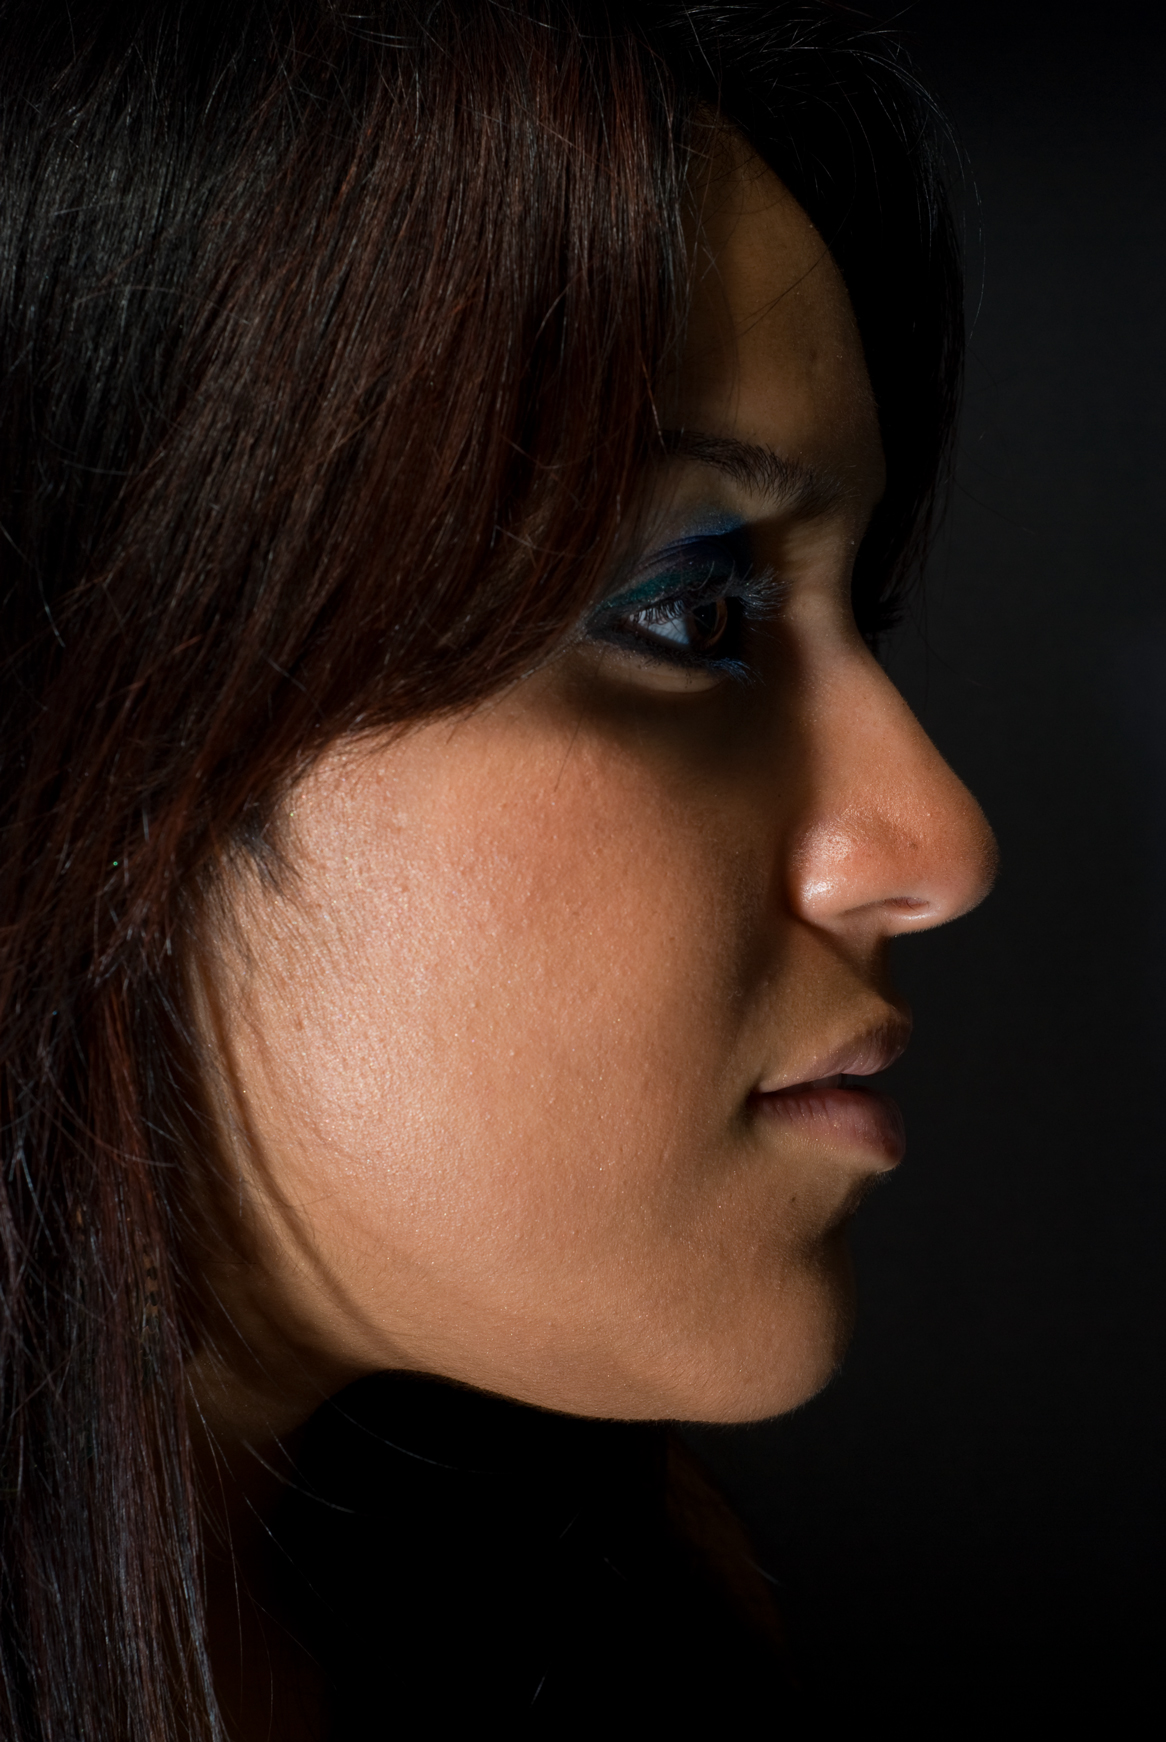
\includegraphics[height=0.22\linewidth]{images/AFLW_profile_dark}
\end{center}
\end{minipage}

\end{xpsectionbox}

